\paragraph{QuizziPedia::Front-End::Models::QuestionnaireModel}
		
		\label{QuizziPedia::Front-End::Models::QuestionnaireModel}
		
		\begin{figure}[ht]
			\centering
			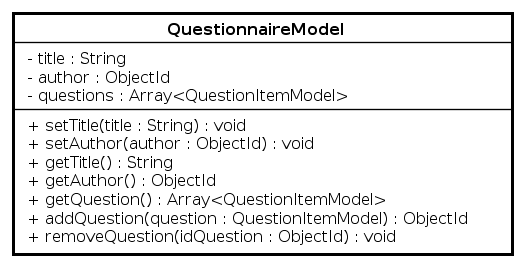
\includegraphics[scale=0.5,keepaspectratio]{UML/Classi/Front-End/QuizziPedia_Front-end_Models_QuestionnaireModel.png}
			\caption{QuizziPedia::Front-End::Models::QuestionnaireModel}
		\end{figure} \FloatBarrier
		
		\begin{itemize}
			\item \textbf{Descrizione}: rappresenta un questionario. Contiene tutte le informazioni necessarie alla presentazione del contenuto del questionario;
			\item \textbf{Utilizzo}: viene utilizzata per memorizzare i dati di un questionario;
			\item \textbf{Relazioni con altre classi}: 
			\begin{itemize}
				\item \textit{IN} \texttt{SearchController}: questa classe permette di gestire la ricerca di questionari e utenti all'interno dell'applicazione;
				\item \textit{IN} \texttt{QuestionnaireDetailsController}: questa classe permette di gestire tutti i questionari creati da un utente; 
				\item \textit{IN} \texttt{FillingQuestionnaireController}: questa classe permette di gestire la creazione e la modifica di una domanda a riempimento di spazi;
				\item \textit{IN} \texttt{CreateQuestionnaireController}: questa classe permette di gestire la creazione di un questionario;
				\item \textit{IN} \texttt{RegistrationManagementController}: questa classe permette di gestire le iscrizione degli utenti ai questionari;
				\item \textit{IN} \texttt{ResultsController}: questa classe permette di gestire i risultati della ricerca effettuata dall'utente;
			\end{itemize}
			\item \textbf{Attributi}: 
			\begin{itemize}
				\item \texttt{- title: String}\\
				Questo attributo rappresenta il titolo del questionario;
				\item \texttt{- author: ObjectId}\\
				Questo attributo rappresenta l'autore del questionario;
				\item \texttt{- questions: Array[QuestionItemModel]}\\
				Questo attributo contiene l'\texttt{array} di \texttt{QuestionItemModel} che rappresenta le domande di un questionario;
			\end{itemize}
			\item \textbf{Metodi}: 
			\begin{itemize}
				\item \texttt{+ setTitle(title: String): void} \\
				Metodo \textit{setter\ped{G}} per il titolo del questionario.\\
				\textbf{Parametri}:
				\begin{itemize}
					\item {title: String}\\
					Questo parametro contiene il titolo del questionario. 
				\end{itemize}
				
				\item \texttt{+ setAuthor(author: ObjectId): void} \\
				Metodo \textit{setter\ped{G}} per il campo dati \texttt{author}\\
				\textbf{Parametri}:
				\begin{itemize}
					\item {author: ObjectId}\\
					Questo parametro rappresenta l'autore che ha creato la domanda.
				\end{itemize}
				
				\item \texttt{+ getTitle(): String} \\
				Metodo \textit{getter\ped{G}} che restituisce il titolo del questionario;
				
				\item \texttt{+ getAuthor(): ObjectId} \\
				Metodo \textit{getter\ped{G}} che restituisce il campo dati \texttt{author};
				
				\item \texttt{+ getQuestion(): Array[QuestionItemModel]} \\
				Metodo \textit{getter\ped{G}} che restituisce il campo dati \texttt{questions};
				
				\item \texttt{+ addQuestion(question: QuestionItemModel): ObjectId} \\
				Metodo per aggiungere una domanda all'\texttt{array} di domande.\\
				\textbf{Parametri}:
				\begin{itemize}
					\item {question: QuestionItemModel}\\
					Questo parametro rappresenta la domanda da inserire.
				\end{itemize}
				
				\item \texttt{+ removeQuestion(idQuestion: ObjectId): void} \\
				Metodo per poter eliminare una domanda dal questionario.\\
				\textbf{Parametri}:
				\begin{itemize}
					\item {idQuestion: ObjectId}\\
					Questo parametro rappresenta l'id della domanda che si vuole rimuove dal questionario.
				\end{itemize}
				
				
			\end{itemize}
		\end{itemize}	
		
		